\section{Experimentation and Results}

Vehicle detection experiments in this study were centered on a 6-class taxonomy 
designed to support emissions-oriented analysis. Several preliminary configurations 
were explored during early development, but those runs were primarily used to 
understand the difficulty of the task and refine the problem formulation. Thus,
the results presented in this section focus on experiments conducted under the 
final 6-class setting. 

First, YOLO-based experiments are presented, including comparisons across model
variants and refinements through data-centric strategies such as hard negative 
mining and dataset refinement. Other detectors like DETR-based models and Faster
R-CNN were examined to compare architectures within the project’s context. 

After identifying the strongest detector, additional experiments evaluate its 
robustness through threshold and NMS sensitivity analysis, cross-camera generalization,
and agreement between predicted vehicle counts and reference ATR or manual counts. 
Together, these experiments exhibit the practical suitability of the final system 
for traffic-monitoring applications.

% ==============================================================================

\subsection{MOVES-based Taxonomy}

For the experiments reported in this chapter, model training and evaluation were 
conducted using a final 6-class taxonomy: 
\verb|passenger_car|, \verb|passenger_truck|, \verb|light_commerical_vehicle|, 
\verb|bus|, \verb|truck|, and \verb|motorcycle|. 
This label set was selected to provide a practical balance between compatibility
with downstream MOVES-based emissions analysis and what could be distinguished 
reliably from low-resolution traffic-camera imagery. Rather than reproducing the
full MOVES source-type framework, the taxonomy preserves broad categories relevant 
to emissions modeling while reducing visual distinctions that are difficult to 
learn consistently.

To achieve this balance, fine-grained vehicle labels were grouped accordingly. 
Sedan instances were mapped to \verb|passenger_car|, while \verb|SUV| instances, 
\verb|pickup_truck| instances, and \verb|van| instances with the attribute \verb|is_minivan| 
instances were grouped into \verb|passenger_truck|. The EPA notes that it is 
difficult to visually determine whether a vehicle should be treated as a 
passenger car or a light-duty truck, but classifies many SUVs and minivans as 
light-duty trucks rather than passenger cars \cite{USEPA_def_truck_2019}. 

The remaining van instances were mapped to \verb|light_commercial_vehicle|. 
This separation is useful from a computer-vision standpoint, as commercial vans 
tend to have more consistent shapes and usage patterns than SUVs and pickup trucks.
It also aligns with MOVES technical guidance, which treats passenger trucks and 
light commercial vehicles as separate source types \cite{USEPA_moves3_2020}. 
Additionally, since the original \verb|two_wheeler| class only contained 
motorcycles, it was remapped directly to \verb|motorcycle|.

Finally, \verb|bus| and \verb|truck| were preserved as independent classes because they are 
operationally different, visually distinct, and treated as separate categories 
within MOVES. Within the bus category, however, school buses were not modeled 
as a separate detector class, even though MOVES distinguishes other buses, 
transit buses, and school buses as separate source types. Instead, school buses
were retained as an annotation attribute and grouped into the broader bus class. 
This is because the primary objective of this study is to identify the broad 
vehicle categories most relevant to downstream emissions-oriented analysis rather
than to infer every possible subtype within each category. As such, the bus 
attribute, \verb|is_school|, was preserved as useful annotation metadata and a potential
avenue for future refinement, but it was not treated as essential to the core 
detector taxonomy. The final mapping between the dataset taxonomy and the MOVES 
taxonomy is shown below in Figure~\ref{fig:moves-taxonomy}.

\begin{figure}[!htbp]
    \centering
    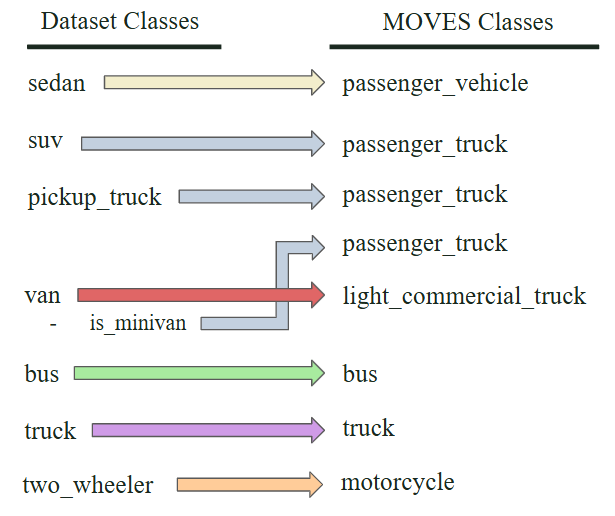
\includegraphics[height=7cm]{figures/results/5_1_class_taxonomy.png}
    \caption{Final MOVES-based class mapping used in this study. Dataset classes 
         on the left were mapped to the MOVES-aligned detector classes on the 
         right. Arrows of the same color indicate the corresponding class 
         mapping, with van instances labeled \texttt{is\_minivan} grouped into 
         \texttt{passenger\_truck} and the remaining van instances mapped to 
         \texttt{light\_commercial\_truck}.}
    \label{fig:moves-taxonomy}
\end{figure}

This MOVES-based taxonomy was used for the remainder of the study as the common 
label mapping for the dataset and for all subsequent training, testing, and evaluation.

% ==============================================================================
